%--------------------------------------
% Create title frame
\titleframe

%--------------------------------------
% Table of contents
%\begin{frame}{Overview}
%  \setbeamertemplate{section in toc}[sections numbered]
%  \tableofcontents[hideallsubsections]
%\end{frame}



%--------------------------------------

\begin{frame}{Syllabus}

\begin{columns}
  \begin{column}{0.35\textwidth}
  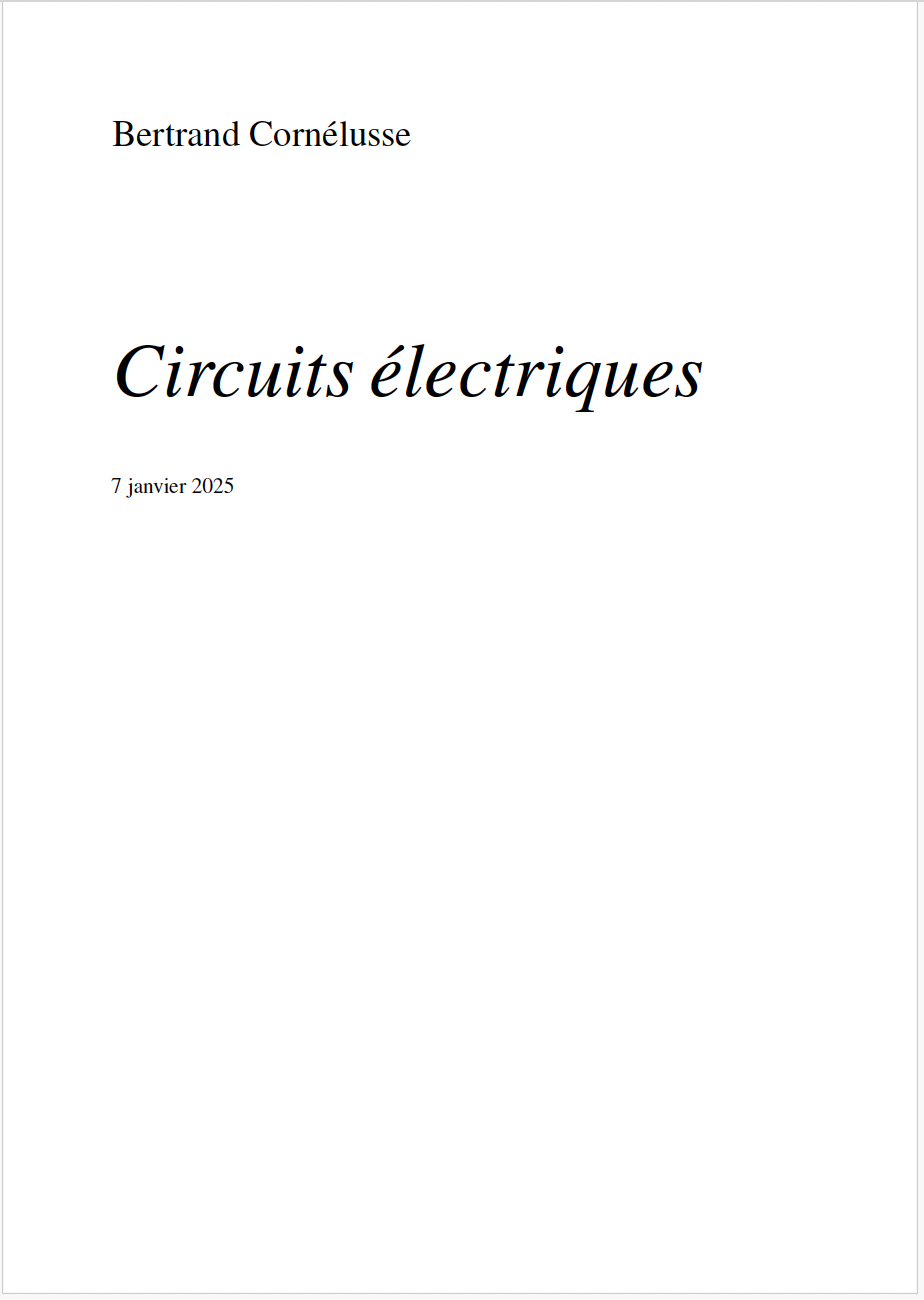
\includegraphics[width=\textwidth]{images/pic_syllabus.png}
  \end{column}
  \begin{column}{0.55\textwidth}
    \begin{itemize}
      \item Version 3 de Janvier 2025
      \item \alert{Nouvelle version bientôt} uniquement pour les expériences (Radio AM avec Bastien Ewbank)
      \item \href{https://github.com/bcornelusse/livre_circuits_electriques_ELEC0053/releases/tag/v3.0}{\underline{\alert{Disponible en ligne}}}
      \item Contient théorie \& exercices
      \item Exercices et résolutions chapitre par chapitre.
    \end{itemize}
  \end{column}
\end{columns}
\end{frame}


\begin{frame}{Communications}

\begin{columns}
  \begin{column}{0.45\textwidth}
    Via \alert{e-Campus}
    \begin{itemize}
      \item Slides : essentiellement des extraits du syllabus. Le syllabus suffit, il contient en réalité (un peu) plus d’information que ce que j’ai le temps de couvrir aux séances
      \item Enregistrement des leçons et des exercices (des années 2020 et 2021) + unicast 2024
      \item Organisation
      \item Compléments ...
      \item Forum
    \end{itemize}
  \end{column}
  \begin{column}{0.45\textwidth}
    Via \alert{GradeScope}
    \begin{itemize}
      \item Résultats d’interros et examen
    \end{itemize}
  \end{column}
\end{columns}
\end{frame}

\begin{frame}{Ce que j’attends de vous}

Séances de théorie et expériences, 13h45 à 15h30, Bertrand Cornélusse, Bastien Ewbank:
\begin{itemize}
  \item Préparez le cours théorique avant la séance, lisez le syllabus ou regardez les vidéos à disposition
  \item \alert{Interagissez}, participez aux activités Wooclap, etc.
\end{itemize}

Séances d’exercices, 15h45 à 17h45, (Thomas Stegen, Guillaume De Bauw, Jolan Lodomez)
\begin{itemize}
  \item Travaillez en groupes et avec les assistant·e·s pour résoudre les exercices par vous-mêmes
  \item Solutions dans le syllabus et dans les vidéos, vous pouvez les regarder à votre aise quand bon vous semble
  \item Posez vos questions sur le forum ou lors des séances de Q{\&}A avant les interros
\end{itemize}
\end{frame}

\begin{frame}{Évaluation - Examen écrit}
Sessions de Juin et d’Aout : 
  \begin{itemize}
    \item Partie Théorie (1h15):  
    \begin{itemize}
      \item une question QROL (\alert{dans une liste de questions})
      \item questions QROC, vrai/faux, QCM
    \end{itemize}
    \item Partie Exercices (2h30)	
    \begin{itemize}
      \item 3 exercices du type de ceux réalisés aux TP
      \item \alert{Calculatrice nécessaire !}
      \item formulaire d’une page A4 recto-verso autorisé
    \end{itemize}
    \item \textbf{Pondération : Théorie 35 \%, Exercices 65 \%}
  \end{itemize}

 

\end{frame}

\begin{frame}{Évaluation - Interros}

2 interrogations bonus pendant le quadrimestre 
\begin{itemize}
  \item facultatives, interviennent pour environ 61 % de la note « Exercices » de juin (donc 40% de la note finale) 
  \item si réalisées toutes les deux, 
  \item et si font monter la note
  \item \alert{calculatrice nécessaire !}
  \item formulaire d’une page A4 recto-verso autorisé

\end{itemize}

\end{frame}

\begin{frame}{Précisions pour le formulaire et la calculatrice}

\begin{columns}
  \begin{column}{0.45\textwidth}
    Le \alert{formulaire} doit être limité à une page A4 recto-verso. Il peut contenir toute information qui vous semble utile.
  \end{column}
  \begin{column}{0.45\textwidth}
    \alert{Calculatrice} : il n'y a pas de restriction particulière sur le modèle, du moment qu'on ne tombe pas dans la catégorie smartphone ou ordinateur portable.
    Apprenez à être à l'aise pour manipuler \alert{les nombres complexes}.

  \end{column}
\end{columns}
\end{frame}

\begin{frame}{Réponses aux questions}
\begin{columns}
  \begin{column}{0.45\textwidth}
    En dehors de la plage du cours, merci de passer par le forum \alert{e-campus} dédié. Nous ne répondrons pas aux questions posées par un autre canal

  \end{column}
  \begin{column}{0.45\textwidth}
    Si vous souhaitez une entrevue, merci de préférer la plage du cours ou de prendre RDV pendant celle-ci.
  \end{column}
\end{columns}
\end{frame}


\begin{frame}{Planning}

Voir le document partagé : \\
\url{https://docs.google.com/spreadsheets/d/17hhljjxt8yALf5o23L1yzglrCsgHS1O-7ts26mENWP0/edit?usp=sharing}

\end{frame}